\documentclass[a4paper,12pt]{report}
\usepackage[backend=biber]{biblatex}
\addbibresource{reference.bib}
\usepackage[hidelinks]{hyperref}
\usepackage{float}
\usepackage{graphicx}
\usepackage{listings}
\usepackage[utf8]{inputenc}
\usepackage{etoolbox}
\usepackage{fullpage}
\renewcommand*\contentsname{Indice}
\renewcommand{\lstlistingname}{Listato}
\usepackage{setspace}
\usepackage{parskip}
\usepackage{amsmath}

% un po' di estetica...
\usepackage{fancyhdr}
\pagestyle{fancy}
\setlength{\headsep}{0.35in}
\let\MakeUppercase\relax

% blocchi di codice
\usepackage{listings}
\lstset{
	breaklines=true, 
	frame=single, 
	numbers=left,
	tabsize=2,
	basicstyle=\scriptsize,
	showstringspaces=false,
	language=C++
}

\setlength{\parindent}{2em}
\setlength{\parskip}{0.5em}
\renewcommand{\baselinestretch}{1.5}

\fancyhf{} % clear all fields
\fancyfoot[C]{\thepage}

\frenchspacing

\newcommand{\mychapter}[2]{
    \setcounter{chapter}{#1}
    \setcounter{section}{0}
    \chapter*{#2}
    \addcontentsline{toc}{chapter}{#2}
}

\begin{document}

\begin{titlepage}
\noindent
    \vspace*{5mm}
	\begin{minipage}[t]{0.15\textwidth}
	    \vspace*{5mm}
		\vspace{-3.5mm}{
\includegraphics[scale=1.8]{../img/logo_bicocca.png}}
	\end{minipage}
	\hspace{1cm}
	\begin{minipage}[t]{0.9\textwidth}
	      \vspace*{5mm}
		{
			\setstretch{1.42}
			{\textsc{Università degli Studi di Milano - Bicocca} } \\
			\textbf{Scuola di Scienze} \\
			\textbf{Dipartimento di Informatica, Sistemistica e Comunicazione} \\
			\textbf{Corso di Laurea Magistrale in Informatica} \\
			\par
		}
	\end{minipage}
	
	\vspace{42mm}

\begin{center}
    {\LARGE{
	    	\setstretch{2}
            \textbf{
            	Metodi del Calcolo Scientifico - Progetto 2 \\ 
            	Compressione di immagini tramite la DCT \\ }
    }}        
\end{center}

\vspace{40mm}
	
	
	\begin{flushright}
		\setstretch{1.3}
		\large{Alberici Federico - 808058\\} 
		\large{Bettini Ivo Junior - 806878\\} 
		\large{Cocca Umberto - 807191\\} 
		\large{Traversa Silvia - 816435} 
	\end{flushright}
	
	\vspace{15mm}
	\begin{center}
		{\large{\bf Anno Accademico 2019 - 2020}}
	\end{center}


\renewcommand{\baselinestretch}{1.5}

\end{titlepage}

\tableofcontents

\mychapter{0}{Introduzione}
In questa relazione vengono presentate e discusse le modalita di implementazione della DCT (dall'inglese Discrete Cosine Transform), ovvero la più diffusa funzione che provvede alla compressione spaziale.\\
Nella prima parte viene confrontata la versione nativa delle DCT implementata in questo progetto con alcune varianti fast (FFT), studiandone il costo computazionale.\\   %"Nativa" della DCT con alcune varianti conosciute, studiandone il costo computazionale.\\
Nella seconda parte viene documentato un semplice tool per applicare su immagini in toni di grigio, tramite un approccio di compressione di tipo jpeg (senza utilizzare una matrice di quantizzazione), la funzione DCT2 implemetata. %in teoria dobbiamo usare quella della libreria (fast)


\mychapter{1}{Analisi DCT}

\section{Discrete Cosine Transform}
Una DCT esprime una sequenza finita di punti in termini di una somma di funzioni coseno oscillanti a diverse frequenze. Ad oggi è una delle tecniche di trasformazione piu utlizzate nella Teoria dei segnali e nella compressione dei dati, in particolare nei media digitali (audio, video, radio ecc..).\\
In queste applicazioni infatti la maggior parte delle informazioni significative tendono ad essere concentrate in poche componenti a bassa frequenza della DCT. Questo permette di comprimere a piacere il dato scartando le componenti ad alta frequenza (compressione lossy).

\section{DCT e IDCT}
La DCT-II è probabilmente la forma più utilizzata, infatti viene indicata come "la DCT".\\
\[C_k = \alpha_k \sum_{i=0}^{N-1} V_i\cos \left[\frac{\pi \left(2i + 1\right) k }{2N}\right] \quad i = 0, \dots, N-1 \quad e \quad \alpha_k = \begin{cases} 1/\sqrt{N}, & \mbox{se } k\mbox{ = 0} \\ \sqrt{2/N}, & \mbox{se } \mbox{\(1 \leq k \leq N - 1\)} \end{cases}\]\\\\
La sua inversa è la DCT-III e per questo viene indicata come "l'inversa della DCT" o "IDCT".\\
\[V_i = \sum_{k=0}^{N-1} \alpha_k C_k \cos \left[\frac{\pi \left(2i + 1\right) k }{2N}\right] \quad k = 0, \dots, N-1 \quad e \quad \alpha_k = \begin{cases} 1/\sqrt{N}, & \mbox{se } k\mbox{ = 0} \\ \sqrt{2/N}, & \mbox{se } \mbox{\(1 \leq k \leq N - 1\)} \end{cases}\]\\\\

Entrambe le funzioni effettuano N somme per calcolare la k-esima componente di un vettore di N componenti, determinando un costo computazionale \( O(N^2)\).

\subsection*{Implementazione}
Per l'implementazione è stato utilizzato C++, sfruttando la libreria open-source Eigen (\url{https://eigen.tuxfamily.org/}) per semplificare la gestione dei dati.\\
\begin{lstlisting}[caption={Funzione di calcolo DCT},captionpos=b]
	void DCT2::DCT(Eigen::VectorXd &_v)
	{
	
		const Eigen::VectorXd _v_copy = _v;
		const int N = _v.size();
		double ak = 1.0 / sqrt(N);
		double ck = 0;
	
		for (int k = 0; k < N; k++)
		{
			ck = 0;
			for (int i = 0; i < N; i++)
			{
				ck += cos((2.0 * i + 1.0) * k * M_PI / (2.0 * N)) * _v_copy(i);
			}
			_v(k) = ak * ck;
			if (k == 0)
			{
				ak = sqrt(2.0) / sqrt(N);
			}
		}
	}
\end{lstlisting}
\hfill \break
\begin{lstlisting}[caption={Funzione di calcolo IDCT},captionpos=b]
void DCT2::IDCT(Eigen::VectorXd &_c)
{
    const Eigen::VectorXd _c_copy = _c;
    const int N = _c.size();
    double ak = 0;
    double vi = 0;

    for (int i = 0; i < N; i++)
    {
        vi = 0;
        ak = 1.0 / sqrt(N);
        for (int k = 0; k < N; k++)
        {
            vi += cos((2.0 * i + 1.0) * k * M_PI / (2.0 * N)) * _c_copy(k) * ak;
            if (k == 0)
            {
                ak = sqrt(2.0) / sqrt(N);
            }
        }
        _c(i) = vi;
    }
}
\end{lstlisting}

\section{DCT2 e IDCT2}
La DCT2 è una trasformazione a due dimensioni, ottenuta semplicemente applicando la DCT mono-dimensionale ad una dimensione, seguita da un'altra applicazione all'altra dimensione.\\
La definizione della DCT bi-dimensionale per una matrice A \textit{m x n} in input è:\\
\begin{align*}
C_{kl} = \alpha_k \alpha_l \sum_{i=0}^{m-1} \sum_{j=0}^{n-1}&A_{ij} \cos \left[\frac{\pi \left(2i + 1\right) k }{2m}\right] \cos \left[\frac{\pi \left(2j + 1\right) l }{2n}\right],\\
&con \quad 0 \leq k \leq m - 1, \quad 0 \leq l \leq n - 1,\\
&\alpha_k = \begin{cases} 1/\sqrt{m}, & \mbox{se } i\mbox{ = 0} \\ \sqrt{2/m}, & \mbox{se } \mbox{\(1 \leq i \leq m - 1\)} \end{cases} \quad e \quad \alpha_l = \begin{cases} 1/\sqrt{n}, & \mbox{se } j\mbox{ = 0} \\ \sqrt{2/n}, & \mbox{se } \mbox{\(1 \leq j \leq n - 1\)} \end{cases}
\end{align*}
L'inversa di tale trasformazione è la IDCT2, ottenuta applicando IDCT alle due dimensioni.

\subsection*{Implementazione}
Anche in questo caso Eigen è utilizzato per mantenere la struttura dati tramite un oggetto \textit{Eigen::MatrixXd}. L'implementazione non sfrutta direttamente la definizione ma computa la DCT2/IDCT2 prima sulle righe e poi sulle colonne della matrice in input. Inoltre essendo l'elaborazione di ogni vettore indipendente dagli altri è possibile parallelizzarne la computazione.\\
\begin{lstlisting}[caption={Funzione di calcolo DCT2},captionpos=b]
	Eigen::MatrixXd DCT2::DCT2_mt(Eigen::MatrixXd &_m)
	{
		Eigen::MatrixXd out = _m;
	
	// DCT su righe
	#pragma omp parallel for
		for (int i = 0; i < out.rows(); i++)
		{
			Eigen::VectorXd row = out.row(i);
			DCT(row);
			out.row(i) = row;
		}
	
	// DCT su colonne
	#pragma omp parallel for
		for (int i = 0; i < out.cols(); i++)
		{
			Eigen::VectorXd col = out.col(i);
			DCT(col);
			out.col(i) = col;
		}
	
		return out;
	}
\end{lstlisting}
\newpage
\begin{lstlisting}[caption={Funzione di calcolo IDCT2},captionpos=b]
	Eigen::MatrixXd DCT2::IDCT2_mt(Eigen::MatrixXd &_m)
	{
		Eigen::MatrixXd out = _m;
	
	// IDCT su righe
	#pragma omp parallel for
		for (int i = 0; i < out.rows(); i++)
		{
			Eigen::VectorXd row = out.row(i);
			IDCT(row);
			out.row(i) = row;
		}
	
	// IDCT su colonne
	#pragma omp parallel for
		for (int i = 0; i < out.cols(); i++)
		{
			Eigen::VectorXd col = out.col(i);
			IDCT(col);
			out.col(i) = col;
		}
	
		return out;
	}
\end{lstlisting}

\section{Varianti DCT}
Esistono diverse varianti della DCT che riducono la complessita a \(O(NlogN)\). Tali metodi sono conosciuti come \textit{fast DCT} o \textit{FCT} in quanto appunto migliorano notevolmente il costo computazionale.\\Di seguito vengono citate due delle più comuni.

\subsubsection*{Fast DCT di Lee}
Descritta da Byeong Gi Lee \cite{Lee} nel 1984 è uno degli algoritmi fast DCT per \(2^m\) punti più comune. Utilizza una struttura ricorsiva dove la trasformazione DCT è decomposta in una parte pari e una dispari. Queste parti sono a loro volta decomposte nello stesso modo finchè non sono abbastanza piccole (N=2) da essere calcolate tramite valutazione diretta \cite{LAGERSTRM2001DesignAI}.

\subsubsection*{Fast DCT FFT}
Invece di applicare direttamente la formula DCT (o scomporla come mostrato da Lee) è possibile fattorizzare la computazione in modo simile alla \textit{fast Fourier transform} (FFT). Gli algoritmi basati su sull'algoritmo di Cooley-Tukey \cite{10.2307/2003354} sono i piu comuni, ma qualunque altro algoritmo FFT è applicabile. 

\section{Confronto}
\begin{figure}[H]
\centering
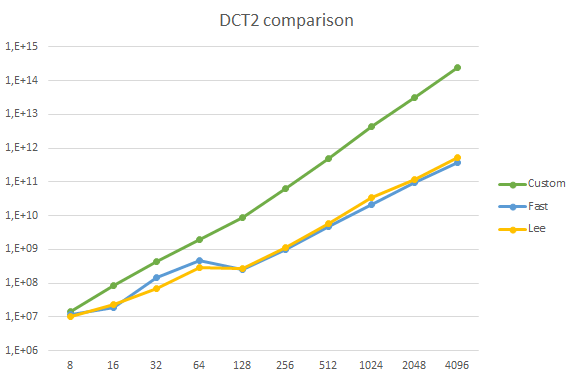
\includegraphics[width=0.77\linewidth]{../img/comparison.png}
\caption{\textit{Confronto DCT2 custom, Fast DCT di Lee e Fast DCT FFT}}
%\label{fig:2}
\end{figure}
Per poter rappresentare graficamente il confronto fra l'algoritmo di DCT2 da noi implementato (\textit{Custom}), l'algoritmo fast della libreria Lee (\textit{Lee}) e l'algoritmo che sfrutta la fast Fourier transform (\textit{Fast}) è stato utilizzato un grafico a linee con indicatori, ponendo sull'asse delle ascisse la dimensione della matrice (sono state utilizzate dimensioni in potenza di 2 per poter eseguire il codice di Lee) e sulle ordinate il tempo impiegato, espresso in scala logaritmica. \\
Si può notare chiaramente che la crescita del tempo impiegato dall'algoritmo Custom è esponenziale rispetto all'andamento similare che hanno gli algoritmi Fast e Lee. %è giusto dire esponenziale? o meglio controllare se effettivamente è O n^3?

\mychapter{2}{Test con immagini}
Il programma è stato scritto tramite QT, una libreria multipiattaforma per lo sviluppo di programmi che utilizzano un'interfaccia grafica (attraverso l'uso di widget) che utlizza il linguaggio C++ (motivo per il quale abbiamo deciso di utilizzarlo).\\
Nella seconda parte del progetto, il programma utilizza le seguenti classi scritte da noi:
\begin{itemize}
\item \textbf{main.cpp}, la quale si occupa di eseguire l'intero corpo del programma;
\item \textbf{compress.cpp}, la quale data un' immagine x esegue delle iterazioni per creare delle sottomatrici che verrano utiliazzate poi dalla libreria dct2 (presa da noi online, da sistemare). Inoltre, una volta che la libreria dct2 esegue il calcolo, questa classe si occupa di ricomporre l'immagine finale;
%\item DCT2.cpp, classe creata ad hoc da noi che implementa la funzione della DCT2 (scrivere meglio);
\item \textbf{mainwindow.cpp}, classe che gestisce tutti gli aspetti e i trigger della interfaccia grafica;
%\item test.cpp, la quale gestisce la parte di confronto generando una matrice randomica che viene eseguita sia da DCT2 e da dct2;
\end{itemize}
Inoltre, viene utilizzata la libreria DCTFast nella quale ricaviamo la DCT2 operando prima per righe e poi per colonne.\\
 
\section{Tool di testing}
Una volta avviato il programma, è possibile caricare l'immagine .bmp tramite un apposito tasto ed inserire i valori di f e d. Una volta inseriti i parametri, tramite il pulsante process viene chiamato il metodo on\_parameters\_clicked(), che dopo aver controllato che f e d rispettino tutti i vincoli trasmorma l'immagine (tramite la funzione pixmapToMatrix()) in una matrice e la invia alla funzione DCTcompress. Questa funzione divide l'immagine in blocchi, applica la DCT2 e poi restituisce una matrice che viene passata alla funzione matrixToPixmap() per poter essere visualizzata in output nell'iterfaccia grafica.\\
La funzione compress prende in input una matrice di interi e i parametri f e d restituendo in output una matrice di interi. Al suo interno, la matrice di input viene trasformata nel formato double e viene eseguito un troncamento per poter scartare gli "avanzi". Iterativamente, per ogn i blocco quadrato f x f applichiamo la dct2 e poi ritorniamo la matrice nel formato int (arrottondando o suoi valori double all'intero più vicino, mettendo a zero i valori negativi e a 255 quelli maggiori di 255). 

\section{Risultati}
Il programma è stato testato sulle immagini di prova fornite e sono stati sperimentati diversi valori dei parametri \textit{F} e \textit{d}. \\

\noindent L'immagine \textit{bridge.bmp} ha dimensione 2749 x 4049, impostando come parametri  \textit{F} = 200 e \textit{d}. = 100 non è visibile alcuna differenza nell'immagine compressa.

\begin{figure}[H]
\centering
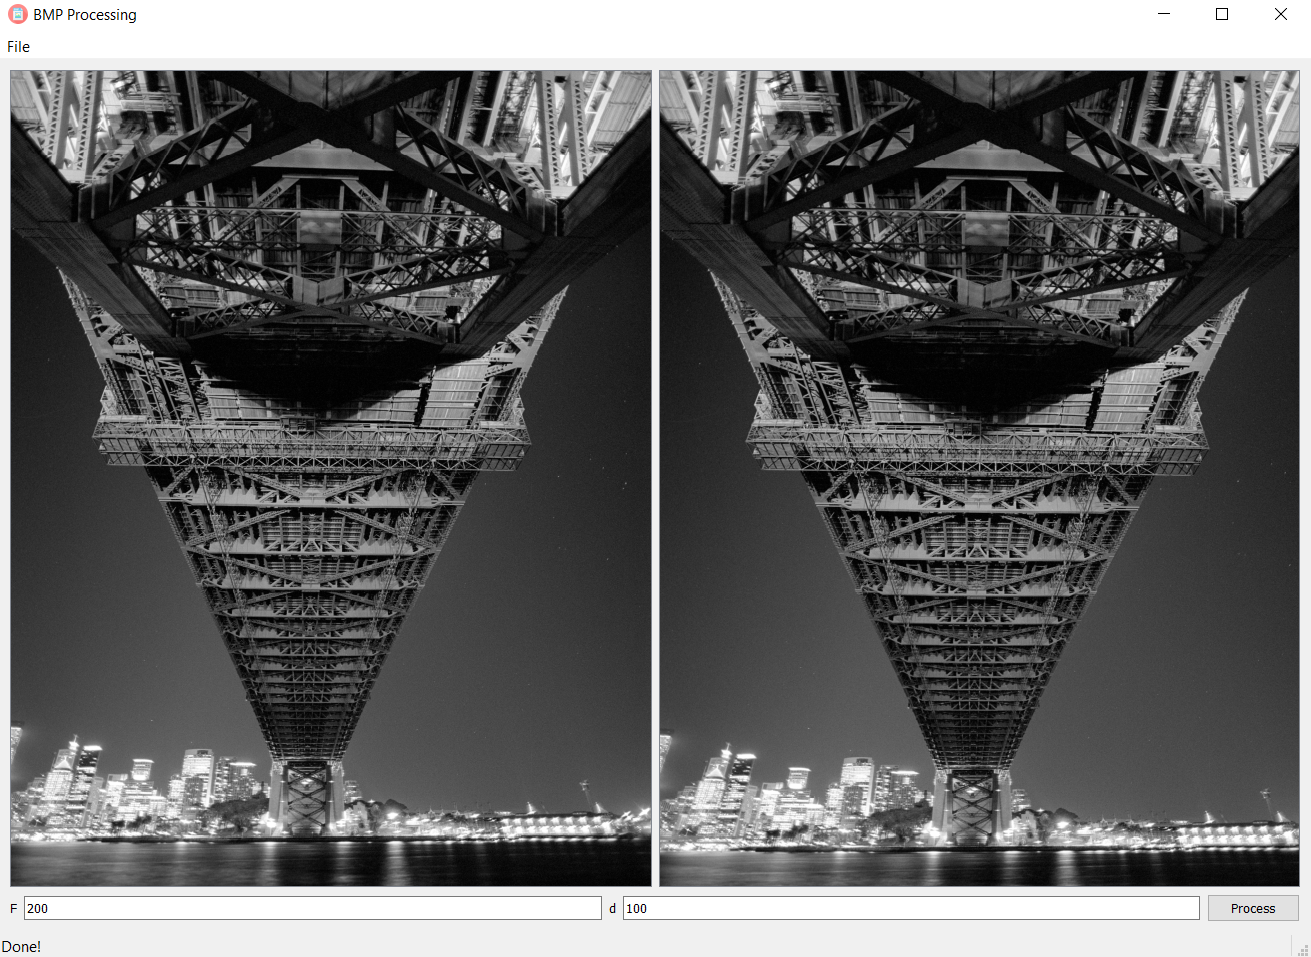
\includegraphics[width=0.8\linewidth]{../img/bridge_200_100.png}
\caption{\textit{bridge.bmp con F = 200 e d = 100}}
\end{figure}

\noindent Tenendo fisso il parametro \textit{F} e diminuendo fortemente il valore del parametro \textit{d}, portandolo a 7, sono visibili ora nell'immagine compressa i blocchi.

\begin{figure}[H]
\centering
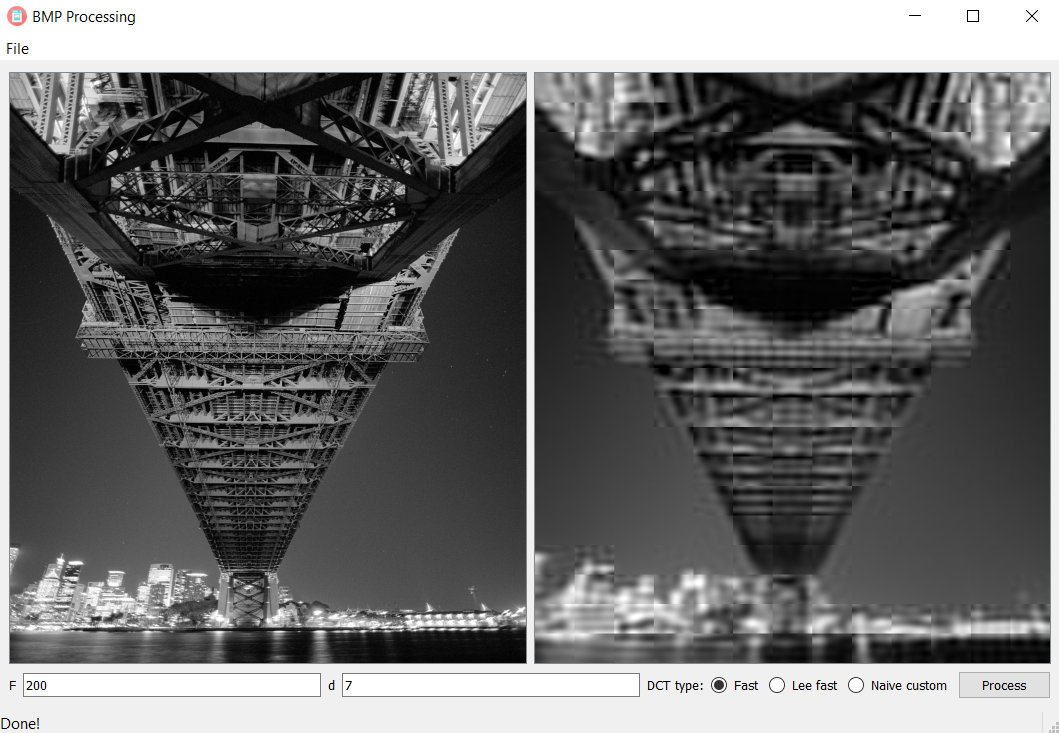
\includegraphics[width=0.8\linewidth]{../img/bridge_200_7.png}
\caption{\textit{bridge.bmp con F = 200 e d = 7}}
\end{figure}

\newpage
\noindent Con l'immagine \textit{deer.bmp}, di dimensione 4043x2641 abbiamo voluto sperimentare con un valore di \textit{F} maggiore, pari a 250, e con valori di \textit{d} bassi.
Impostando \textit{d} = 50 l'immagine risulta lievemente sgranata.

\begin{figure}[H]
\centering
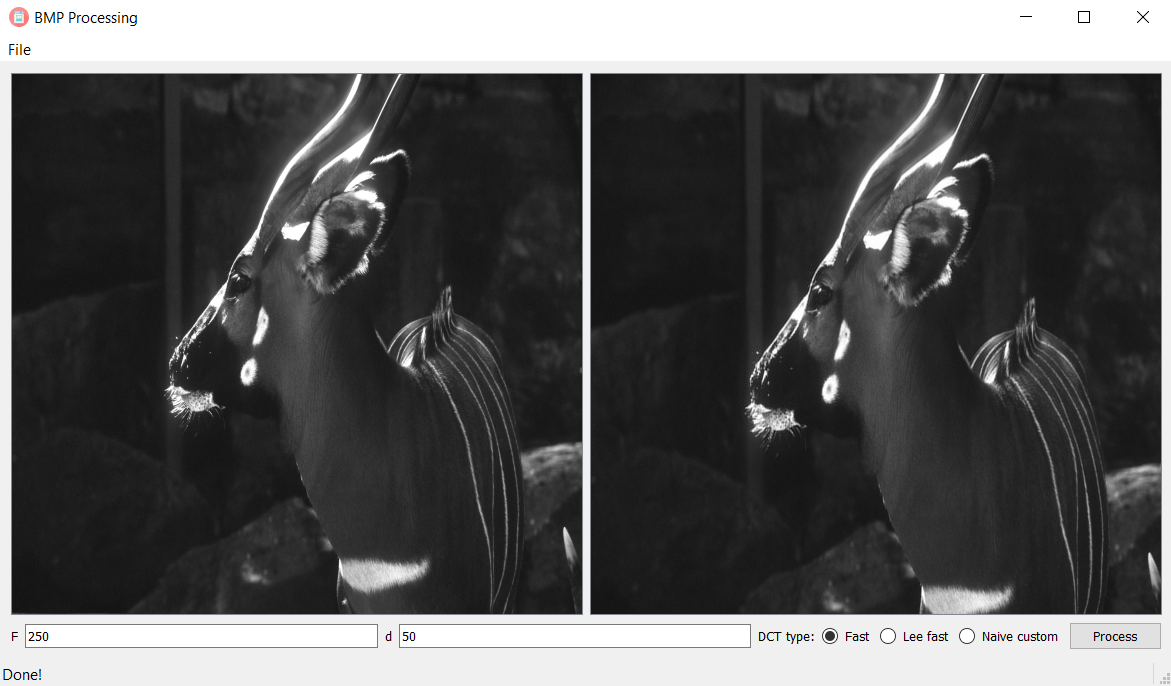
\includegraphics[width=0.8\linewidth]{../img/bambi_250_50.png}
\caption{\textit{deer.bmp con F = 250 e d = 50}}
\end{figure}

Abbassando il valore di \textit{d} a 9 sono visibili i blocchi.

\begin{figure}[H]
\centering
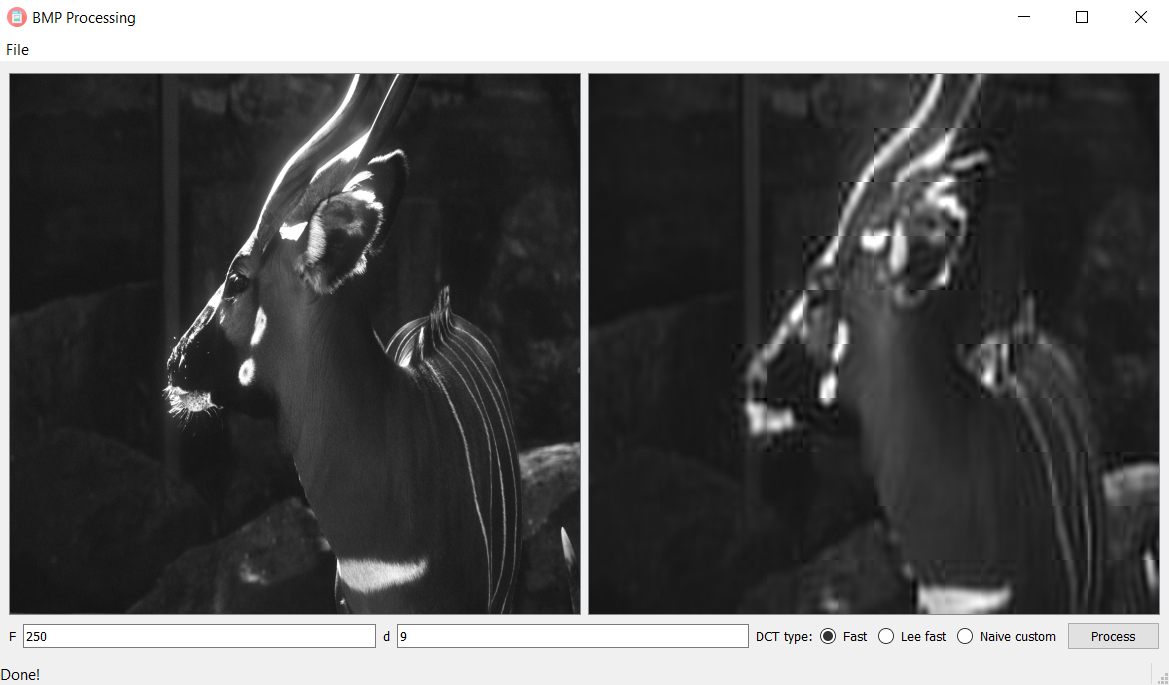
\includegraphics[width=0.8\linewidth]{../img/bambi_250_9.png}
\caption{\textit{deer.bmp con F = 250 e d = 9}}
\end{figure}

\newpage
Per l'immagine \textit{cathedral.bmp} (2000x3008) abbiamo voluto testare valori di \textit{F} piccoli con valori di \textit{d} relativamente vicini.
Ponendo \textit{F} = 20 e \textit{d} = 15 otteniamo un'immagine che non sembra differire dall'originale se non per una luminosità maggiore.

\begin{figure}[H]
\centering
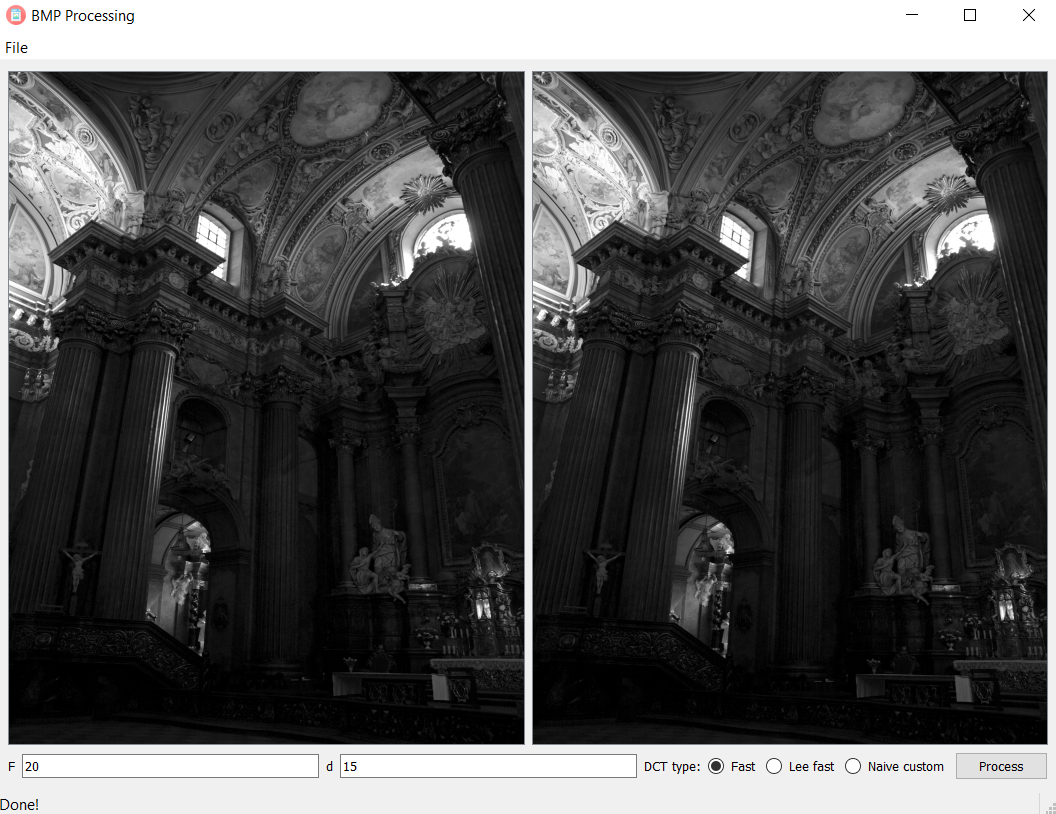
\includegraphics[width=0.8\linewidth]{../img/cathedral_20_15.png}
\caption{\textit{cathedral.bmp con F = 20 e d = 15}}
\end{figure}

Abbiamo successivamente impostato \textit{F} = 10 ed abbiamo assegnato a \textit{d} un valore maggiore, 17. L'immagine risulta pressoché identica.

\begin{figure}[H]
\centering
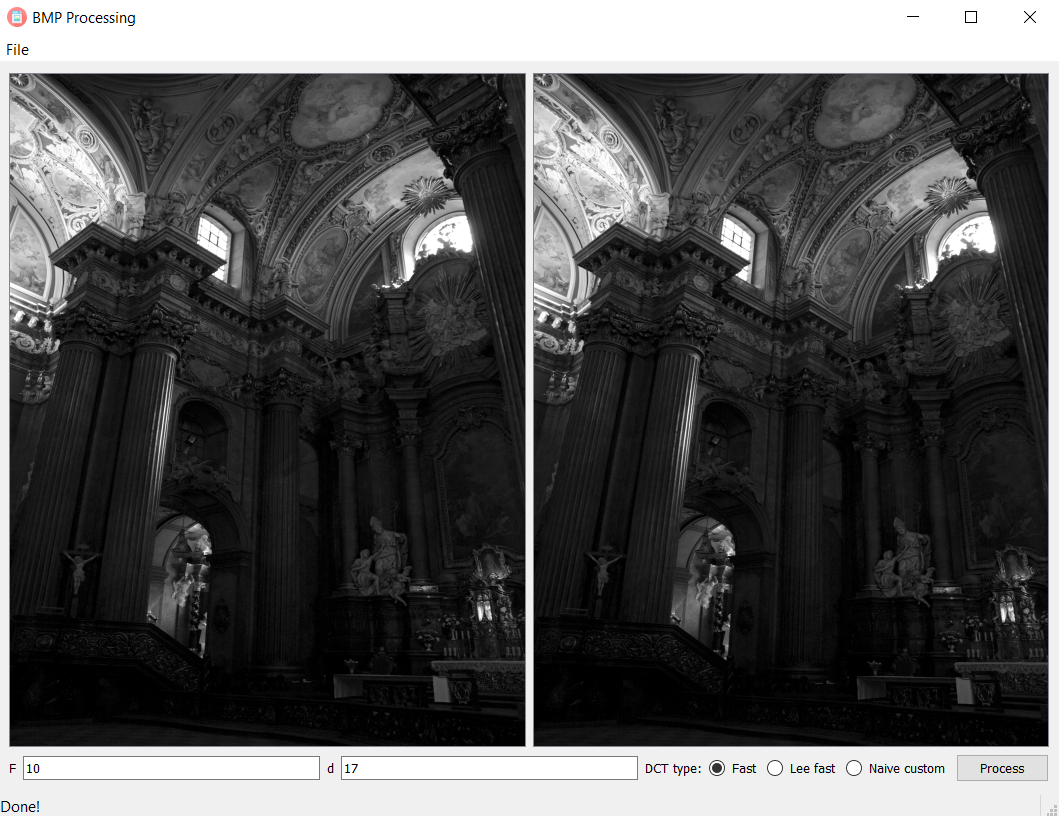
\includegraphics[width=0.8\linewidth]{../img/cathedral_10_17.png}
\caption{\textit{cathedral.bmp con F = 10 e d = 17}}
\end{figure}

\printbibliography

\end{document}